\problemname{Curve Speed}

To help with vehicle stability, the outer edge of a road in a curve
is raised with respect to the inner edge. This is called superelevation
and is specified as the difference in elevation divided by the width 
of the road. It needs to be higher for faster speeds and sharper curves.

The radius of a curve is the radius of the section of a circle along the
middle of the road where the curve is constant. See Figure~1 for a
drawing of this.

\begin{figure}[h]
	\begin{center}
		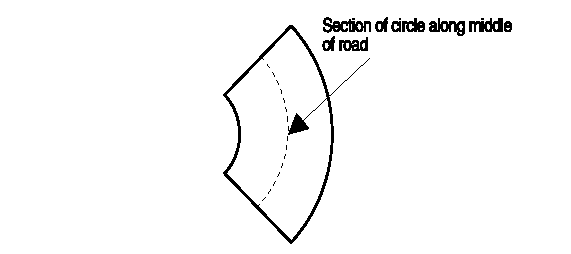
\includegraphics[width=.65\textwidth]{F1CurveSpeed.pdf}
	\end{center}
	\caption{Section of a circle along the middle of a road with radius $R$.}
	\label{fig:1}
\end{figure}

In some cases the curve may need a lower speed limit than straight
portions of the road. The superelevation shouldn't be more than about
$.12$ to keep vehicles from sliding off the road in slippery conditions.

Your job is to calculate the maximum speed on a curve given the radius
of the curve and the superelevation.

The maximum speed is given by this formula:
$$V = \sqrt{(R*(S+.16))/.067},$$
where $V$ is the max speed in miles per hour, $R$ is the radius of the curve
in feet, and S is the superelevation.

\section*{Input}

The input is a series of lines terminated by end-of-file. Each line
will be a test case consisting of $R$ and $S$ separated by whitespace. $R$
will be an integer greater than $99$ and less than $5281$ and $S$ will be a 
real number greater than $.009$ and less than $1.0$. Neither will have 
leading zeros. There are at most $100$ lines in input.

\section*{Output}

For each test case output the maximum speed rounded to the nearest
integer. It is guaranteed the answer before rounding will not be within $10^{-3}$
of a half-integer value.